\documentclass[12pt, a4paper]{article}

% PACKAGES
\usepackage{amsmath}         % For advanced math environments
\usepackage{geometry}        % For setting page margins
\usepackage{tikz}            % For drawing diagrams
\usepackage{amsfonts}        % For math fonts
\usepackage{amssymb}         % For math symbols
\usepackage{tabularx}        % For tables that fit page width

% HYPERREF SETUP (one call to the package with options)
\usepackage[colorlinks=true, linkcolor=blue, urlcolor=blue]{hyperref}

% PAGE GEOMETRY
\geometry{a4paper, margin=1in}

% DOCUMENT INFO
\title{Supplemental Problems in Rotational Dynamics}
\author{}
\date{\today}

\begin{document}

\maketitle
\tableofcontents
\newpage

\section{New Application Problems with Solutions}

\subsection{Problem 1: Potter's Wheel}
\textbf{Problem:} A potter's wheel, a solid uniform disk of mass $M = 20.0$ kg and radius $R = 0.40$ m, is freely rotating about its center at an angular velocity of $15.0 \text{ rad s}^{-1}$. A potter drops a lump of clay of mass $m = 2.5$ kg from just above the wheel, and it sticks to the wheel at a distance $r = 0.30$ m from the center. What is the new angular velocity of the wheel-clay system, and what is the change in its rotational kinetic energy?

\begin{center}
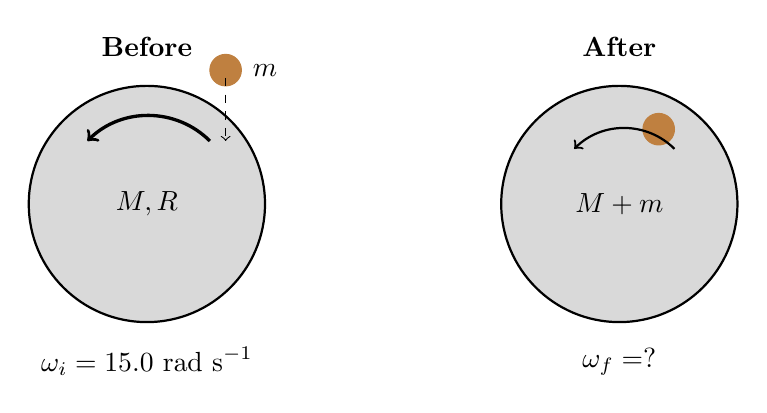
\begin{tikzpicture}
    % Before State
    \begin{scope}[xshift=-3cm]
        \node at (0, 2) {\textbf{Before}};
        % Wheel
        \draw[fill=gray!30, thick] (0,0) circle (1.5);
        \draw[->, very thick] (0.8, 0.8) arc (45:135:1.1);
        \node at (0, 0) {$M, R$};
        \node at (0, -2) {$\omega_i = 15.0 \text{ rad s}^{-1}$};
        % Clay
        \filldraw[brown] (1, 1.7) circle (0.2);
        \node at (1.5, 1.7) {$m$};
        \draw[->, dashed] (1, 1.6) -- (1, 0.8);
    \end{scope}

    % After State
    \begin{scope}[xshift=3cm]
        \node at (0, 2) {\textbf{After}};
        % Wheel with clay
        \draw[fill=gray!30, thick] (0,0) circle (1.5);
        \filldraw[brown] (0.5, 0.95) circle (0.2);
        \node at (0, 0) {$M+m$};
        \draw[->, thick] (0.7, 0.7) arc (45:135:0.9);
        \node at (0, -2) {$\omega_f = ?$};
    \end{scope}
\end{tikzpicture}
\end{center}

\textbf{Explanation:} This problem is an application of the \textbf{conservation of angular momentum}. Since the clay is dropped vertically, it adds no initial angular momentum to the system. The net external torque is zero. However, adding the clay increases the system's total moment of inertia. As a result, the angular velocity must decrease to conserve angular momentum. The kinetic energy is expected to decrease because a non-conservative, inelastic collision occurs when the clay sticks to the wheel.

\textbf{Solution:}
\begin{enumerate}
    \item \textbf{Calculate the initial moment of inertia ($I_i$):} This is just the moment of inertia of the solid disk.
    \[ I_i = I_{disk} = \frac{1}{2}MR^2 = \frac{1}{2}(20.0 \text{ kg})(0.40 \text{ m})^2 = 1.60 \text{ kg m}^2 \]

    \item \textbf{Calculate the final moment of inertia ($I_f$):} This is the sum of the disk's inertia and the inertia of the clay (treated as a point mass).
    \[ I_f = I_{disk} + I_{clay} = \frac{1}{2}MR^2 + mr^2 \]
    \[ I_f = 1.60 \text{ kg m}^2 + (2.5 \text{ kg})(0.30 \text{ m})^2 = 1.60 + 0.225 = 1.825 \text{ kg m}^2 \]

    \item \textbf{Apply conservation of angular momentum to find $\omega_f$:}
    \[ L_i = L_f \implies I_i \omega_i = I_f \omega_f \]
    \[ (1.60 \text{ kg m}^2)(15.0 \text{ rad s}^{-1}) = (1.825 \text{ kg m}^2) \omega_f \]
    \[ \omega_f = \frac{24.0}{1.825} = 13.15 \text{ rad s}^{-1} \]

    \item \textbf{Calculate the change in kinetic energy:}
    \[ K_i = \frac{1}{2} I_i \omega_i^2 = \frac{1}{2}(1.60)(15.0)^2 = 180.0 \text{ J} \]
    \[ K_f = \frac{1}{2} I_f \omega_f^2 = \frac{1}{2}(1.825)(13.15)^2 = 158.0 \text{ J} \]
    \[ \Delta K = K_f - K_i = 158.0 \text{ J} - 180.0 \text{ J} = -22.0 \text{ J} \]
    The rotational kinetic energy decreases by $22.0 \text{ J}$.
\end{enumerate}

\newpage
\subsection{Problem 2: T-Shaped Pendulum}
\textbf{Problem:} A T-shaped pendulum is constructed from two identical uniform rods, each with mass $M = 1.2$ kg and length $L = 0.8$ m. One rod (the "post") hangs vertically from a pivot at its top end. The second rod (the "crossbar") is attached horizontally to the bottom end of the post. A bullet of mass $m = 0.05$ kg is fired horizontally with speed $v = 150 \text{ m/s}$ and strikes the end of the crossbar, embedding itself there. Find the maximum angle $\theta$ the post makes with the vertical after the collision.

\begin{center}
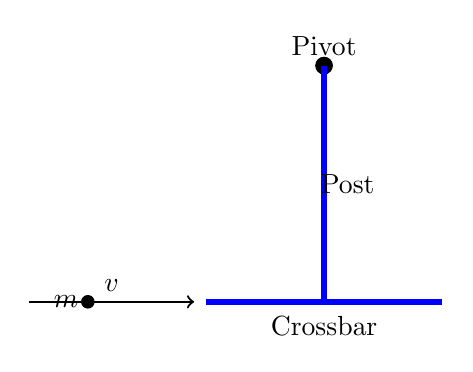
\begin{tikzpicture}[scale=1.5]
    % Pivot
    \filldraw (0,0) circle (2pt) node[above] {Pivot};
    % Vertical Post
    \draw[line width=2pt, blue] (0,0) -- (0, -2);
    % Horizontal Crossbar
    \draw[line width=2pt, blue] (-1, -2) -- (1, -2);
    % Bullet
    \filldraw[black] (-2, -2) circle (1.5pt) node[left] {$m$};
    \draw[->, thick] (-2.5, -2) -- (-1.1, -2) node[midway, above] {$v$};
    \node at (0.2, -1) {Post};
    \node at (0, -2.2) {Crossbar};
\end{tikzpicture}
\end{center}

\textbf{Explanation:} This problem combines several concepts. First, we must calculate the total moment of inertia of the T-shaped object about the pivot, using the \textbf{Parallel Axis Theorem} for both rods. Then, we use \textbf{conservation of angular momentum} for the inelastic collision to find the initial angular velocity of the system. Finally, we use \textbf{conservation of mechanical energy} (rotational kinetic to potential) during the subsequent swing to find the maximum angle. This requires finding the center of mass of the final system.

\textbf{Solution:}
\begin{enumerate}
    \item \textbf{Calculate the system's moment of inertia ($I_{sys}$) about the pivot:}
    \begin{itemize}
        \item Post rod (pivot at end): $I_{post} = \frac{1}{3}ML^2 = \frac{1}{3}(1.2)(0.8)^2 = 0.256 \text{ kg m}^2$.
        \item Crossbar (Parallel Axis Theorem): Its CM is at distance $d=L=0.8$ m from the pivot.
        \[ I_{cross} = I_{cm} + Md^2 = \frac{1}{12}ML^2 + ML^2 = \frac{13}{12}ML^2 \]
        \[ I_{cross} = \frac{13}{12}(1.2)(0.8)^2 = 0.832 \text{ kg m}^2 \]
        \item Bullet (after sticking): It strikes at a distance $r = \sqrt{L^2 + (L/2)^2} = \sqrt{0.8^2 + 0.4^2} = 0.894$ m from the pivot.
        \[ I_{bullet} = mr^2 = (0.05)(0.894)^2 = 0.040 \text{ kg m}^2 \]
        \item Total: $I_{sys} = I_{post} + I_{cross} + I_{bullet} = 0.256 + 0.832 + 0.040 = 1.128 \text{ kg m}^2$.
    \end{itemize}
    \item \textbf{Apply conservation of angular momentum for the collision:}
    The bullet's lever arm is $r_{\perp} = L = 0.8$ m.
    \[ L_i = r_{\perp} (mv) = (0.8 \text{ m})(0.05 \text{ kg})(150 \text{ m/s}) = 6.0 \text{ kg m}^2\text{s}^{-1} \]
    \[ L_f = I_{sys} \omega_f \implies 6.0 = 1.128 \omega_f \implies \omega_f = 5.32 \text{ rad s}^{-1} \]

    \item \textbf{Apply conservation of energy for the swing:}
    First, find the initial position ($y_{CM}$) of the system's center of mass below the pivot.
    \[ y_{CM} = \frac{M(L/2) + M(L) + m(L)}{M+M+m} = \frac{1.2(0.4) + 1.2(0.8) + 0.05(0.8)}{1.2+1.2+0.05} = \frac{1.48}{2.45} = 0.604 \text{ m} \]
    Now, conserve energy: $K_i = U_f$. The change in height is $\Delta h_{CM} = y_{CM}(1-\cos\theta)$.
    \[ \frac{1}{2} I_{sys} \omega_f^2 = (M_{tot}) g \Delta h_{CM} \]
    \[ \frac{1}{2} (1.128) (5.32)^2 = (2.45)(9.81)(0.604)(1-\cos\theta) \]
    \[ 15.96 = 14.51(1-\cos\theta) \]
    \[ 1-\cos\theta = \frac{15.96}{14.51} = 1.10 \]
    \textbf{Result Analysis:} A value of $(1-\cos\theta) > 1$ is physically impossible. This means the pendulum has enough energy to swing all the way over the top. The greatest angle with the downward vertical would be $180^\circ$ as it passes through the top point.
\end{enumerate}

\newpage
\subsection{Problem 3: Composite Disc Roll}
\textbf{Problem:} A composite wheel is made of a solid aluminum disc ($M_{Al}=4.0$ kg, $R_{in}=0.2$ m) and a concentric steel ring ($M_{St}=6.0$ kg) of outer radius $R_{out}=0.3$ m. The wheel is released from rest at the top of a ramp of height $h=2.5$ m. Assuming it rolls without slipping, what is the translational speed of its center of mass at the bottom of the ramp?

\begin{center}
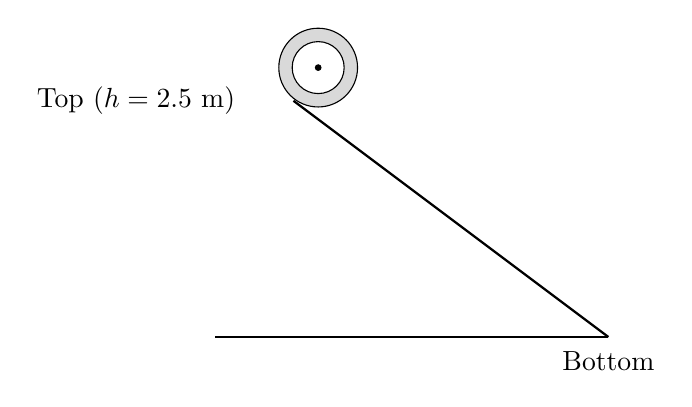
\begin{tikzpicture}
    % Ramp
    \draw[thick] (0,3) -- (4,0); % The slope
    \draw[thick] (4,0) -- (-1,0); % The ground
    \node at (-2, 3.0) {Top ($h=2.5$ m)};
    \node at (4, -0.3) {Bottom};
    
    % *** CORRECTED WHEEL POSITION ***
    % The wheel is now correctly placed at the top of the ramp.
    \begin{scope}[xshift=0.4, yshift=3.45]
        \draw[fill=gray!30] (0.3,3.3) circle (0.5); % Outer radius
        \draw[fill=white] (0.3,3.3) circle (0.33); % Inner radius scaled for drawing
        \filldraw (0.3,3.3) circle (1pt);
    \end{scope}
\end{tikzpicture}
\end{center}

\textbf{Explanation:} This problem uses \textbf{conservation of mechanical energy} for a rolling object. The initial potential energy of the wheel at the top of the ramp is converted into both translational and rotational kinetic energy at the bottom. The key is to first calculate the total moment of inertia for the composite object (disc + ring) about its center.

\textbf{Solution:}
\begin{enumerate}
    \item \textbf{Calculate the total moment of inertia ($I_{CM}$):}
    This is the sum of the inertia of the inner disc and the outer ring.
    \begin{itemize}
        \item Inner disc: $I_{Al} = \frac{1}{2} M_{Al} R_{in}^2 = \frac{1}{2}(4.0)(0.2)^2 = 0.08 \text{ kg m}^2$.
        \item Outer ring: $I_{St} = \frac{1}{2} M_{St} (R_{out}^2 + R_{in}^2) = \frac{1}{2}(6.0)(0.3^2 + 0.2^2) = 3.0(0.09+0.04) = 0.39 \text{ kg m}^2$.
        \item Total: $I_{CM} = I_{Al} + I_{St} = 0.08 + 0.39 = 0.47 \text{ kg m}^2$.
    \end{itemize}

    \item \textbf{Apply conservation of energy:}
    The total mass is $M_{tot} = M_{Al} + M_{St} = 4.0 + 6.0 = 10.0$ kg. The condition for rolling without slipping is $\omega = v_{CM}/R_{out}$.
    \[ E_{top} = E_{bottom} \]
    \[ U_g = K_{trans} + K_{rot} \]
    \[ M_{tot} g h = \frac{1}{2} M_{tot} v_{CM}^2 + \frac{1}{2} I_{CM} \omega^2 \]
    Substitute $\omega = v_{CM}/R_{out}$:
    \[ M_{tot} g h = \frac{1}{2} M_{tot} v_{CM}^2 + \frac{1}{2} I_{CM} \left(\frac{v_{CM}}{R_{out}}\right)^2 \]
    \[ M_{tot} g h = \frac{1}{2} v_{CM}^2 \left( M_{tot} + \frac{I_{CM}}{R_{out}^2} \right) \]
    Plug in the values:
    \[ (10.0)(9.81)(2.5) = \frac{1}{2} v_{CM}^2 \left( 10.0 + \frac{0.47}{0.3^2} \right) \]
    \[ 245.25 = \frac{1}{2} v_{CM}^2 (10.0 + 5.22) \]
    \[ 245.25 = \frac{1}{2} v_{CM}^2 (15.22) \]
    \[ v_{CM}^2 = \frac{2 \times 245.25}{15.22} = 32.23 \]
    \[ v_{CM} = \sqrt{32.23} = 5.68 \text{ m s}^{-1} \]
\end{enumerate}

\newpage
\subsection{Problem 4: Hanging Door Collision}
\textbf{Problem:} A uniform wooden door of mass $M=15$ kg, height $H=2.0$ m, and width $w=0.8$ m is hanging at rest from its hinges. A ball of clay with mass $m=0.5$ kg is thrown horizontally and strikes the door perpendicular to its surface at its center, sticking to it. If the door swings through a maximum angle of $\theta = 30^\circ$, what was the initial speed $v$ of the clay?

\begin{center}
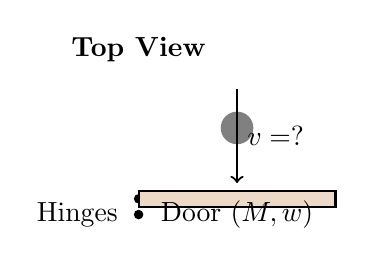
\begin{tikzpicture}
    % Top view of the door and collision
    \node at (0, 2) {\textbf{Top View}};
    % Hinges
    \filldraw (0,0.1) circle (1.5pt);
    \filldraw (0,-0.1) circle (1.5pt) node[left=4pt] {Hinges};
    % Door
    \draw[fill=brown!30, thick] (0,0) rectangle (2.5, 0.2);
    \node at (1.25, -0.1) {Door ($M, w$)};
    % Clay
    \filldraw[gray] (1.25, 1) circle (0.2);
    \draw[->, thick] (1.25, 1.5) -- (1.25, 0.3) node[midway, right]{$v=?$};
\end{tikzpicture}
\end{center}

\textbf{Explanation:} This is the reverse of a typical collision problem. We are given the final state (the maximum swing angle) and must work backward to find the initial state (the clay's speed). We'll start by using \textbf{conservation of mechanical energy} for the swing to find the angular velocity just after the collision. Then, we'll use \textbf{conservation of angular momentum} for the collision to find the initial speed of the clay.

\textbf{Solution:}
\begin{enumerate}
    \item \textbf{Use conservation of energy for the swing to find $\omega$ after collision:}
    The system's rotational kinetic energy just after impact is converted into gravitational potential energy at the peak of the swing. The door can be treated as a uniform plate rotating about an axis on its edge.
    \[ K_i = U_f \implies \frac{1}{2} I_{sys} \omega^2 = M_{tot} g \Delta h_{CM} \]
    First, find the moment of inertia and center of mass of the door-clay system.
    \begin{itemize}
        \item Door (plate pivoted at edge): $I_{door} = \frac{1}{3}Mw^2 = \frac{1}{3}(15)(0.8)^2 = 3.2 \text{ kg m}^2$.
        \item Clay (point mass at center): $I_{clay} = m(w/2)^2 = (0.5)(0.4)^2 = 0.08 \text{ kg m}^2$.
        \item Total: $I_{sys} = 3.2 + 0.08 = 3.28 \text{ kg m}^2$.
    \end{itemize}
    Now, find the system's center of mass distance from the hinges.
    \[ x_{CM} = \frac{M(w/2) + m(w/2)}{M+m} = \frac{(15+0.5)(0.4)}{15+0.5} = 0.4 \text{ m} \]
    The change in height is $\Delta h_{CM} = x_{CM}(1-\cos\theta)$.
    \[ \frac{1}{2} (3.28) \omega^2 = (15.5)(9.81)(0.4)(1-\cos 30^\circ) \]
    \[ 1.64 \omega^2 = (60.82)(1 - 0.866) = (60.82)(0.134) = 8.15 \]
    \[ \omega^2 = \frac{8.15}{1.64} = 4.97 \implies \omega = 2.23 \text{ rad s}^{-1} \]
    This is the angular velocity right after the collision.

    \item \textbf{Apply conservation of angular momentum for the collision:}
    \[ L_i = L_f \]
    The initial angular momentum is provided entirely by the clay, with a lever arm of $w/2$.
    \[ L_i = r_{\perp} (mv) = (w/2)mv = (0.4) (0.5) v = 0.2 v \]
    The final angular momentum is that of the rotating system.
    \[ L_f = I_{sys} \omega = (3.28)(2.23) = 7.31 \text{ kg m}^2\text{s}^{-1} \]
    Equating them:
    \[ 0.2 v = 7.31 \]
    \[ v = \frac{7.31}{0.2} = 36.6 \text{ m s}^{-1} \]
\end{enumerate}

\end{document}